\subsection{Xây dựng mô-đun nhận diện ký hiệu}

Nếu Chương 2 tập trung vào việc lý giải vì sao chọn MediaPipe Holistic và mô hình TFLite pre-trained
(Kaggle ASL Signs), thì phần này mô tả cách mô-đun đã được hiện thực thành mã nguồn cụ thể. Ở
snapshot hiện tại, module nhận diện được tổ chức gọn trong thư mục \texttt{external/asl_baseline/},
bao gồm file mô hình, bảng ánh xạ nhãn và script suy luận thời gian thực.

\subsubsection{Cấu trúc mã nguồn của mô-đun}

\begin{table}[H]
\centering
\caption{Các file chính của mô-đun nhận diện}
\label{tab:recognition-files}
\begin{tabularx}{\textwidth}{|>{\raggedright\arraybackslash}p{5.4cm}|X|}
\hline
\textbf{File} & \textbf{Vai trò} \\
\hline
\codepath{external/asl_baseline/realtime_asl_250.py} & Chương trình webcam thời gian thực: khởi tạo TFLite Interpreter, đọc camera, duy trì sliding window landmarks, suy luận mô hình và hiển thị top-k dự đoán. \\
\hline
\codepath{external/asl_baseline/model.tflite} & Trọng số mô hình đã huấn luyện sẵn, giải pháp đạt giải nhất cuộc thi Kaggle ASL Signs. Kích thước $\sim$11 MB. \\
\hline
\codepath{external/asl_baseline/sign_to_prediction_index_map.json} & Bảng ánh xạ 250 tên từ vựng ký hiệu sang chỉ số đầu ra tương ứng của mô hình. \\
\hline
\codepath{external/asl_baseline/MODEL_README.md} & Tài liệu ghi chú nguồn gốc mô hình và giấy phép MIT. \\
\hline
\end{tabularx}
\end{table}

Cấu trúc này rất gọn so với các mô-đun NLP: toàn bộ logic nhận diện được đóng gói trong một file
Python duy nhất, kèm theo mô hình TFLite và bảng nhãn. Việc sử dụng mô hình pre-trained giúp giảm
đáng kể số lượng file cần quản lý, không cần notebook huấn luyện hay checkpoint riêng.

\subsubsection{Hiện thực trích xuất landmarks bằng MediaPipe}

Lớp \texttt{ASL250Recognizer} trong \texttt{realtime\_asl\_250.py} khởi tạo MediaPipe Holistic với
cấu hình:
\begin{itemize}
    \item \texttt{model\_complexity=1};
    \item \texttt{refine\_face\_landmarks=False};
    \item \texttt{min\_detection\_confidence=0.5};
    \item \texttt{min\_tracking\_confidence=0.5}.
\end{itemize}

Hàm \texttt{\_extract\_frame\_landmarks(results)} là điểm vào quan trọng nhất của tầng thị giác.
Luồng xử lý gồm các bước:
\begin{enumerate}
    \item lấy landmarks khuôn mặt (468 điểm), tay trái (21 điểm), pose (33 điểm) và tay phải
    (21 điểm);
    \item mỗi nhóm landmarks được trải phẳng thành ma trận \texttt{(N, 3)} với tọa độ
    \texttt{(x, y, z)};
    \item nếu thiếu bất kỳ nhóm landmark nào (ví dụ tay không xuất hiện), thay bằng ma trận
    \texttt{NaN} cùng kích thước;
    \item nối bốn nhóm theo thứ tự \texttt{face, left\_hand, pose, right\_hand} thành ma trận
    cuối cùng kích thước \texttt{(543, 3)}.
\end{enumerate}

Thiết kế ``điền NaN khi thiếu landmark'' là một chi tiết kỹ thuật quan trọng, khác biệt so với
phương pháp điền zero thông thường. Giá trị \texttt{NaN} cho phép mô hình TFLite phân biệt rõ
giữa ``không có dữ liệu'' và ``tọa độ bằng 0'', từ đó tránh tạo nhiễu đầu vào không cần thiết.

Thứ tự nối landmarks (face → left\_hand → pose → right\_hand) tuân theo quy ước của cuộc thi
Kaggle ASL Signs và phải được giữ nguyên để đảm bảo tương thích với mô hình pre-trained.

\subsubsection{Hiện thực nạp và suy luận mô hình TFLite}

Trong phương thức khởi tạo, mô hình TFLite được nạp bằng TensorFlow Lite Interpreter.
Quá trình khởi tạo gồm:
\begin{itemize}
    \item nạp file \texttt{model.tflite};
    \item lưu lại chỉ số tensor đầu vào (\texttt{input\_index}) và đầu ra
    (\texttt{output\_index});
    \item nạp bảng ánh xạ nhãn từ \texttt{sign\_to\_prediction\_index\_map.json};
    \item tạo ánh xạ ngược \texttt{id\_to\_sign} để chuyển từ chỉ số sang tên từ vựng.
\end{itemize}

Phương thức \texttt{predict()} thực hiện suy luận theo các bước:
\begin{enumerate}
    \item kiểm tra bộ đệm đã đủ tối thiểu 16 frame chưa;
    \item gom toàn bộ frames trong bộ đệm thành tensor đầu vào;
    \item gọi \texttt{resize\_tensor\_input()} để điều chỉnh kích thước đầu vào theo số frame
    thực tế;
    \item gọi \texttt{allocate\_tensors()}, \texttt{set\_tensor()};
    \item gọi \texttt{invoke()} để chạy suy luận;
    \item lấy kết quả từ \texttt{get\_tensor()};
    \item áp dụng softmax nếu đầu ra chưa ở dạng xác suất;
    \item trả về top-k nhãn có xác suất cao nhất.
\end{enumerate}

Một chi tiết đáng chú ý là hàm \texttt{\_softmax\_if\_needed()}: hàm này kiểm tra xem đầu ra
của mô hình đã ở dạng xác suất (tổng $\approx$ 1, tất cả $\geq$ 0) hay chưa. Nếu chưa, nó tự
động áp dụng softmax. Thiết kế này giúp code hoạt động ổn định bất kể mô hình TFLite trả về
logits hay xác suất.

\subsubsection{Hiện thực suy luận thời gian thực}

Trong phương thức \texttt{run()}, luồng chạy chính của mô-đun nhận diện có thể tóm tắt như sau:
\begin{enumerate}
    \item mở webcam với độ phân giải 960x540;
    \item với mỗi frame: lật ảnh như gương, chuyển sang RGB và xử lý bằng MediaPipe Holistic;
    \item chỉ gom landmarks vào bộ đệm khi phát hiện có bàn tay (trái hoặc phải);
    \item mỗi 8 frame (\texttt{predict\_every=8}), gọi \texttt{predict()} nếu bộ đệm đủ
    16 frame;
    \item hiển thị top-3 dự đoán trên giao diện video;
    \item vẽ skeleton pose và bàn tay lên khung hình bằng MediaPipe drawing utilities.
\end{enumerate}

Từ góc nhìn trải nghiệm người dùng, ba cơ chế nhỏ nhưng hiệu quả là:
\begin{itemize}
    \item \textbf{chỉ gom khi có tay}: lọc các frame không có ý nghĩa ký hiệu;
    \item \textbf{predict\_every = 8}: giảm tải tính toán, không cần suy luận mỗi frame;
    \item \textbf{min\_frames = 16}: đảm bảo mô hình có đủ ngữ cảnh thời gian trước khi
    dự đoán.
\end{itemize}

Hai phím điều khiển chính:
\begin{itemize}
    \item \texttt{Space}: reset bộ đệm và kết quả dự đoán;
    \item \texttt{q}: thoát chương trình.
\end{itemize}

\begin{figure}[H]
\centering
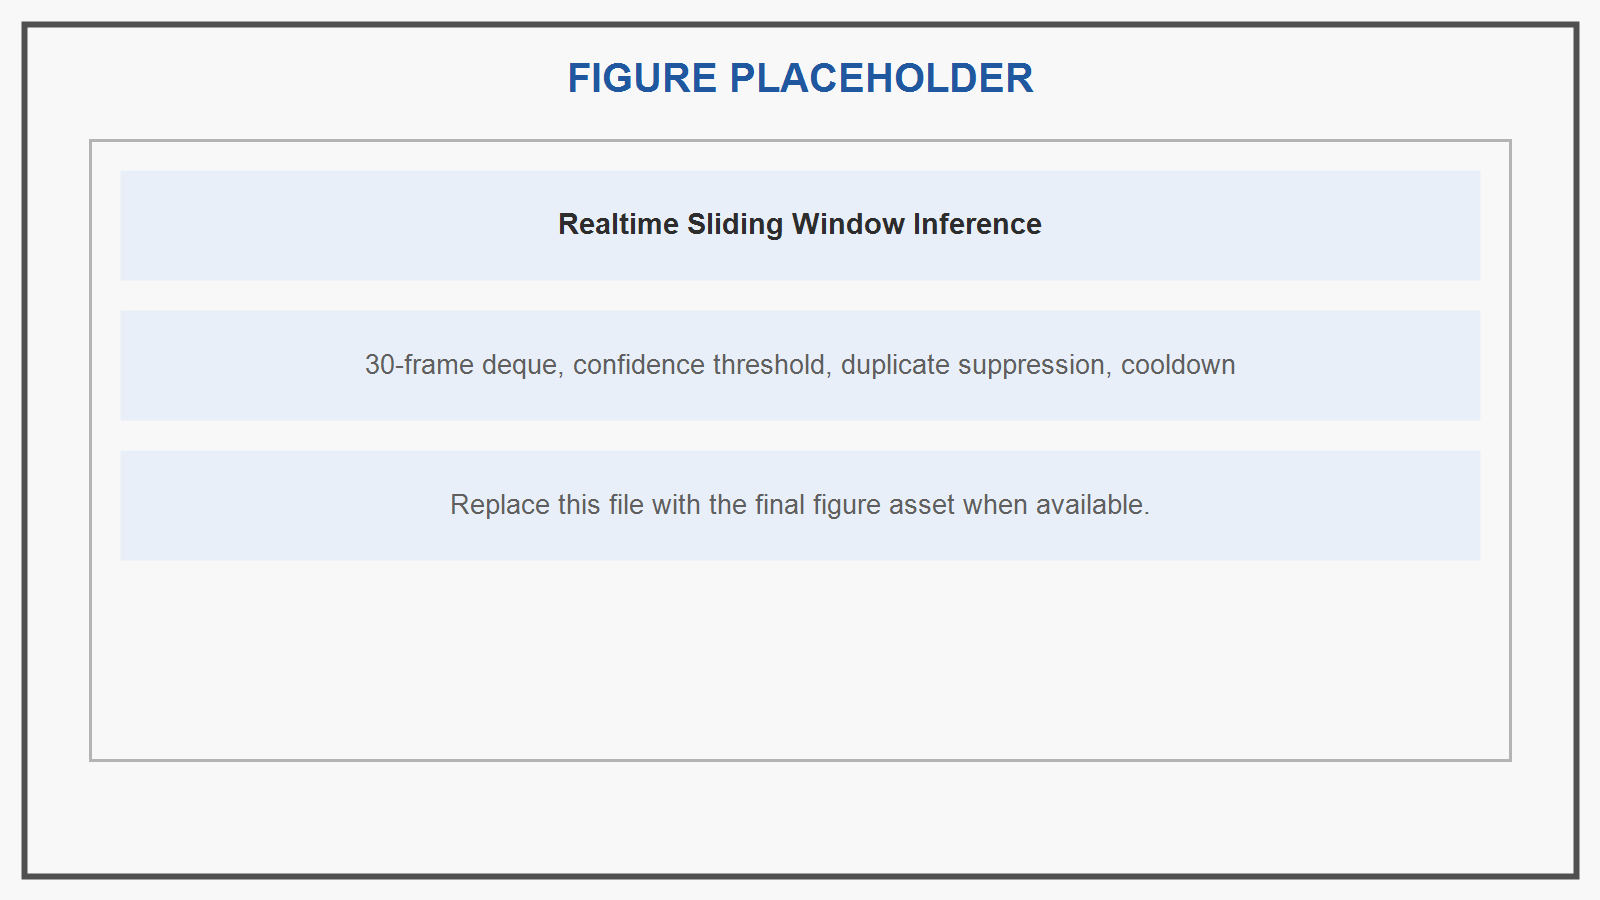
\includegraphics[width=0.84\textwidth]{figures/recognition/realtime_sliding_window.png}
\caption{Sơ đồ sliding window 16--60 frame và logic ``chỉ gom khi có tay'' trong suy luận realtime}
\label{fig:realtime-sliding-window}
\end{figure}

\subsubsection{Nhận xét dưới góc nhìn kỹ thuật phần mềm}

Mô-đun nhận diện hiện tại có nhiều điểm làm tốt ở khía cạnh phần mềm:
\begin{itemize}
    \item toàn bộ logic được đóng gói trong một lớp \texttt{ASL250Recognizer} duy nhất, dễ
    tích hợp và tái sử dụng;
    \item giao diện giữa mô-đun nhận diện và mô-đun NLP chỉ là nhãn gloss, nên dễ tích hợp;
    \item mô hình TFLite chạy trên CPU, không yêu cầu GPU, phù hợp với phần cứng phổ thông;
    \item code hỗ trợ nhiều camera backend (\texttt{CAP\_DSHOW} trên Windows,
    \texttt{CAP\_ANY} trên các hệ điều hành khác);
    \item có argparse để cấu hình camera, max-frames, min-frames từ dòng lệnh.
\end{itemize}

Bên cạnh đó cũng có vài giới hạn cần ghi nhận trung thực trong báo cáo:
\begin{itemize}
    \item phần tích hợp với mô-đun NLP phía sau (ghép câu tiếng Việt, dịch Việt - Lào) chưa
    được nối trực tiếp trong script hiện tại; cần thêm bước ánh xạ gloss tiếng Anh sang token
    tiếng Việt;
    \item vì là mô hình pre-trained, nhóm không thể can thiệp vào kiến trúc bên trong hoặc tinh
    chỉnh thêm cho VSL;
    \item cấu hình hiện tại nhắm tới demo một người, một webcam, chưa phải bài toán nhiều người
    đồng thời hoặc bối cảnh nền phức tạp.
\end{itemize}

Nhìn chung, ở mức đồ án môn học, mô-đun này đã đạt một ngưỡng hiện thực hóa đầy đủ: có mô hình
pre-trained chất lượng cao, có script suy luận realtime và có cổng nối lên tầng NLP thông qua đầu
ra gloss.

